\chapter{Method}

\label{chap:method}

\section{Hardware}
All methods described in this section are implemented and tested on a workstation with the following specifications:
\begin{itemize}[noitemsep]
	\item Operating System: Ubuntu 22.04 LTS
	\item CPU: 13th Gen Intel Core i7-13700K
	\item Graphics card: NVIDIA RTX 4080
	\item RAM: 64 GB DDR5
\end{itemize}

Additionally, custom hardware was used for image data acquisition, which is further detailed in the following section.


\section{Image Acquisition and Tie Points Extraction}

To produce the dataset required for 3D Gaussian Splatting, multiple images of a subject's face from various viewpoints with consistent poses are necessary. A well-composed set of images helps minimize errors in tie point detection and supports a more consistent 3D Gaussian Splatting reconstruction. This section outlines the steps and components for acquiring and preprocessing images as well as extracting tie points.

\subsection{3reCapSL/Photodome Overview}
Data acquisition was conducted using the \href{https://www.uni-weimar.de/de/medien/professuren/medieninformatik/computer-vision/forschung/3d-realitycapture-scanlab/}{3D-RealityCapture-ScanLab} (3reCapSL) by the Computer Vision research group at Bauhaus-Universität, Weimar. The 3reCapSL, often called the Photodome, is a hemispherical structure consisting of 130 consumer DSLR cameras and 130 LED lamps mounted along 12 aluminum arc-shaped columns (as shown in Figure \ref{fig:Photodome}). This arrangement allows for nine circular rows of cameras to be distributed vertically, forming a dome-like structure. The cameras are mounted on the columns using standard camera clamps, enabling stability and adjustability with three degrees of rotational freedom. For this thesis, all cameras used in the Photodome are identical with the following specifications:

\begin{itemize}[noitemsep]
	\item Model: Canon EOS M6 Mark II
	\item Resolution: 6960 pixels wide x 4640 pixels high
	\item Focal Length: 22.0 mm
	\item Pixel Size: 3.2 $\mu$m
	\item Bands: RGB
\end{itemize}

The LED lamps are directed towards the center of the dome and are spaced nearly equidistantly to ensure uniform lighting within the structure. This setup allows for comprehensive coverage of the subject from various viewpoints, capturing images under optimal lighting conditions.

\begin{figure}[H]
	\centering
	\includegraphics[width=0.48\textwidth]{Figures/methods/CV-Lab-Dom.png}
	\includegraphics[width=0.48\textwidth]{Figures/methods/CV-Lab-Dom-Detail.png}
	\caption{Left: The Photodome/3reCapSL with a controller workstation for remote monitoring, data transfer, and camera triggering. Right: A camera mounted on one of the arcs. Credit: \href{https://www.uni-weimar.de/de/medien/professuren/medieninformatik/computer-vision/forschung/computer-vision-labor/c65966}{Laboratory of Computer Vision research group, Bauhaus-University Weimar}}
	\label{fig:Photodome}
\end{figure}

All cameras and LED lamps are connected to a central computer, which triggers the cameras and controls the lamps for a near-simultaneous image capture. The computer also handles image transfer for further processing. 

%As mentioned above, the Photodome is used to capture images of a subject within the structure from various view points covering almost its entire surface. This is followed by a feature extraction process via photogrammetric technique (e.g. stereo matching) to obtain as many feature points as possible across the view and match them. This produces a set of tie points in 3D space also known as a sparse point cloud.

%To clarify, photogrammetry is defined as a study and technology of obtaining reliable information about physical objects and the environment through the process of recording, measuring and interpreting photographic data such as images. The aim of a photogrammetric technique is to provide automatization of this extraction processes as accurately as possible. In order to reliably carry out this process, a photogrammetric software called \href{https://www.agisoft.com/}{\textit{Agisoft Metashape} \texttrademark} is used and installed in the controller workstation. This software is chosen because of its performance and quality of extraction.

%%% COMMENT EICK: I would leave this out all along. That sounds very Wikipedia.

\subsection{Acquisition Details}
\label{sec:acquisition}

For each image acquisition session, the following steps are carried out:
\begin{enumerate}[noitemsep]
	\item The human model takes a seat.
	\item A green screen is set up behind the model.
	\item Adjust the seat height and rotation so the central camera aligns with the models's eye level.
	\item Trigger the cameras.
	\item Transfer images from cameras to the computer.
	\item Resize and center-crop the images.
\end{enumerate}

\begin{figure}[ht]
	\centering
	\begin{subfigure}{0.4\linewidth}
		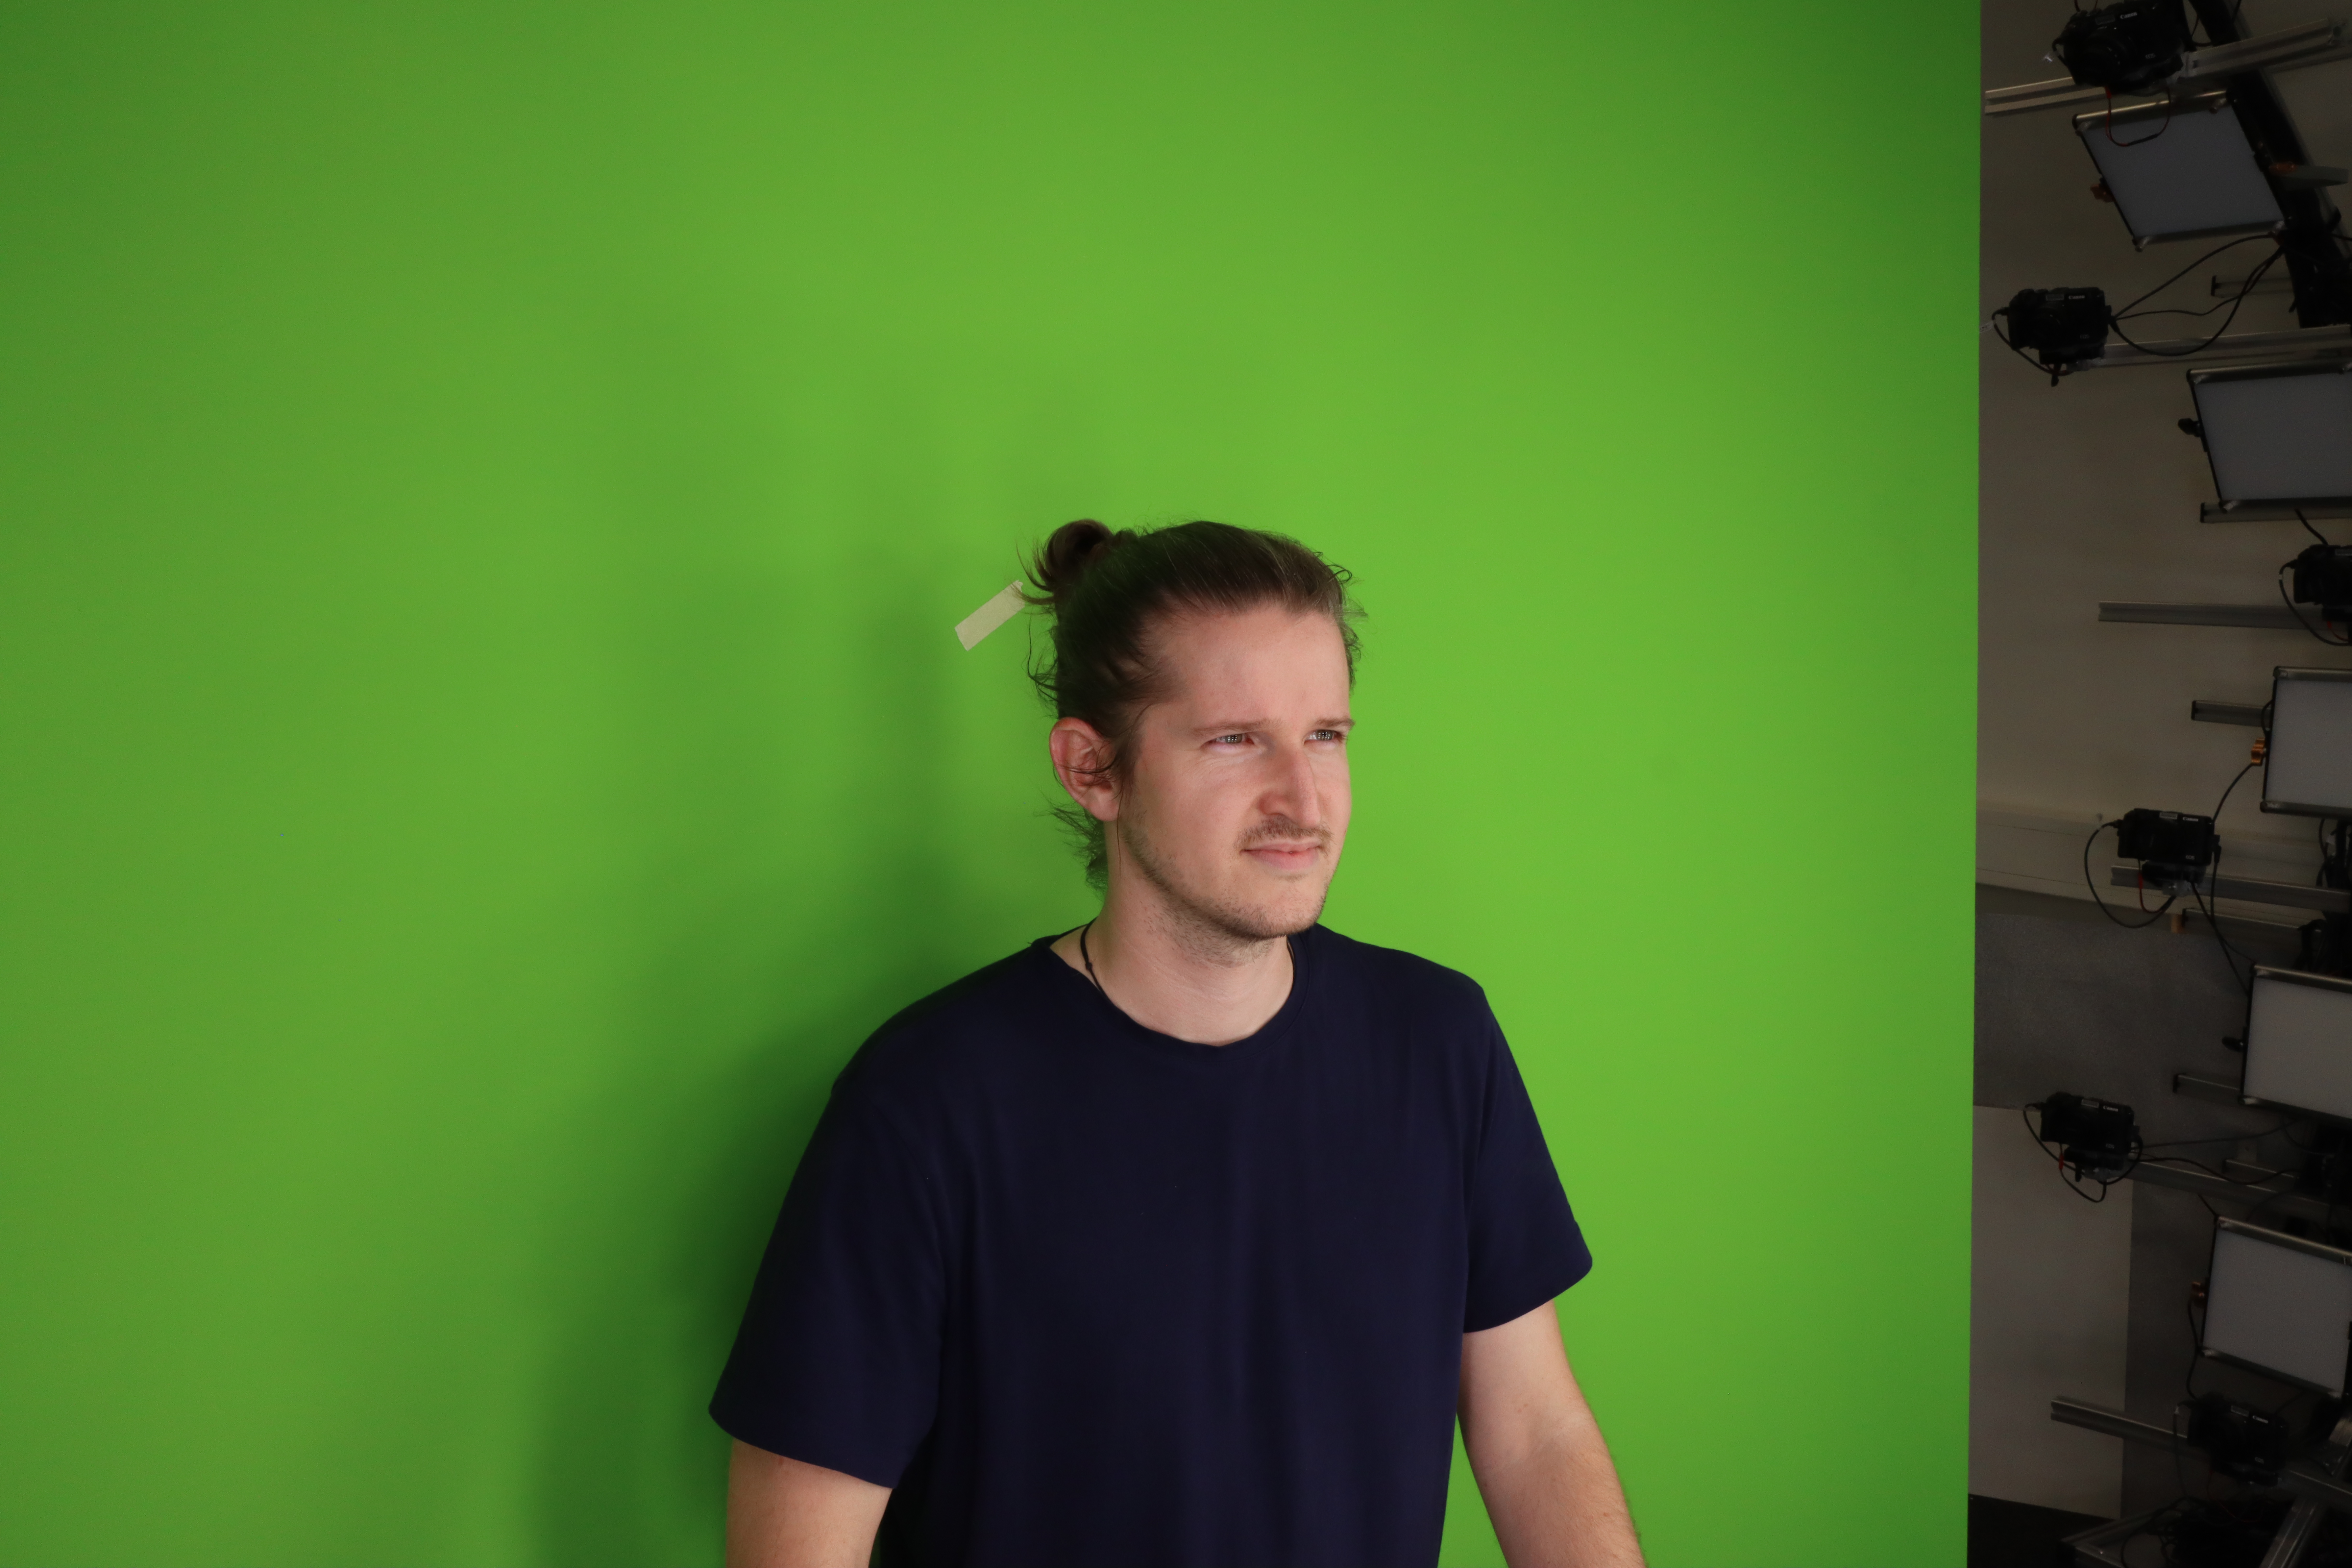
\includegraphics[width=\textwidth]{Figures/methods/6-2-4-2-163452-082_raw.JPG}
		\caption{Raw capture from camera 2-4-2}
	\end{subfigure}
	\begin{subfigure}{0.4\linewidth}
		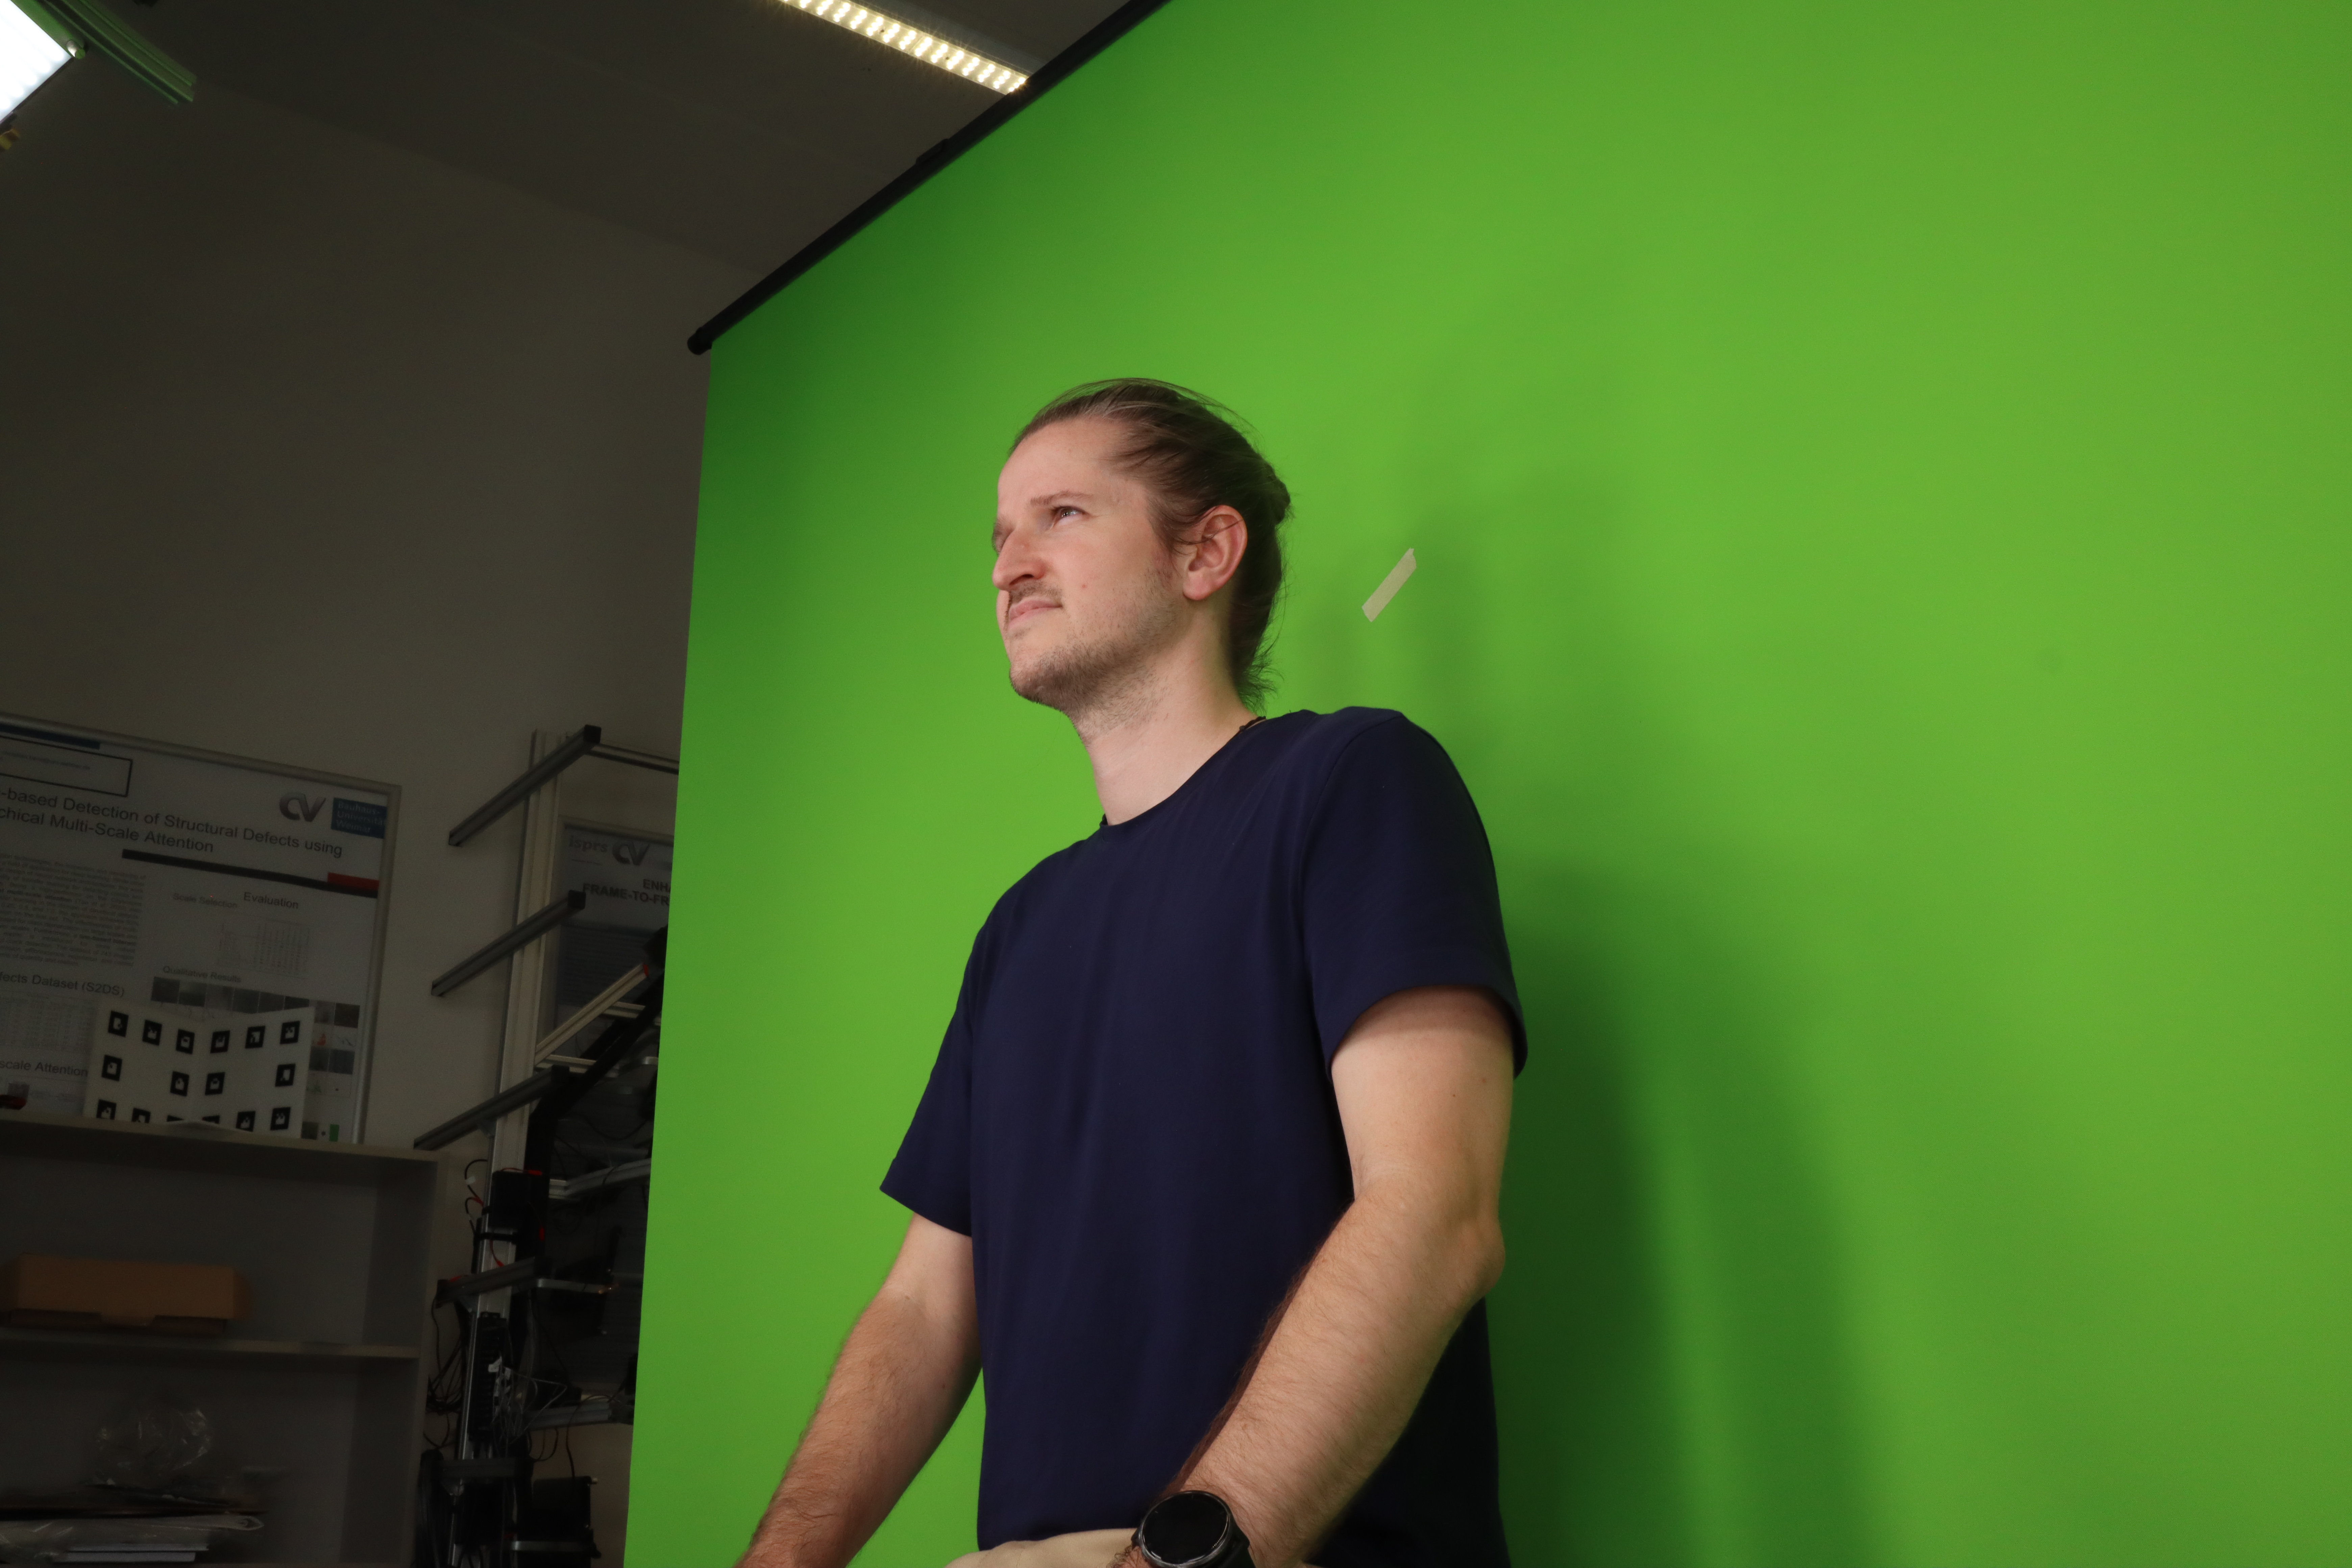
\includegraphics[width=\textwidth]{Figures/methods/6-B-6-2-163452-598_raw.JPG}
		\caption{Raw capture from camera B-6-2}
	\end{subfigure}
	\vfil
	\begin{subfigure}{0.4\linewidth}
		\includegraphics[width=\textwidth]{Figures/methods/6-2-4-2-163452-082_crop.JPG}
		\caption{Cropped capture from camera 2-4-2}
	\end{subfigure}
	\begin{subfigure}{0.4\linewidth}
		\includegraphics[width=\textwidth]{Figures/methods/6-B-6-2-163452-598_crop.JPG}
		\caption{Cropped capture from camera B-6-2}
	\end{subfigure}
	\caption{Raw and cropped images from two different cameras. The masking tape is used to mark the center of the face for the purpose of adjusting the height and rotation of the chair.}
	\label{fig:rawphotodome}
\end{figure}


Since the focus is on stylizing the face, only 37 front-facing cameras are used. Similarly, only the LED lamps directed at the face are activated during capture. These cameras are angled and calibrated to focus primarily on the subject's face, neck, and a small portion of the upper torso. Additionally, a green screen is placed behind the human subject to cover the background and to simplify the extraction of the tie points later on. Since body height varies from person to person, an adjustable chair is used to ensure that the person's eye level aligns with the same camera.
Pictures are taken when the cameras are focused and the human model is ready. Finally, the images are transferred to a computer for resizing. This resizing process ensures that the face and upper torso are centered and occupy a large portion of the image (Figure \ref{fig:rawphotodome}). This step is crucial for ensuring that the stylization functions correctly, as outlined in the documentation of the author's implementation \href{https://github.com/timothybrooks/instruct-pix2pix?tab=readme-ov-file#tips}{usage tips} for InstructPix2Pix \citep{Brooks.2023}. Examples of failed stylization results from earlier experiments during initial research are shown in Figure \ref{fig:unpreprocessed}.


\subsection{Data preparation for 3D Gaussian Splatting}
\label{sec:preprocessing}

Data preprocessing is performed using \textit{Agisoft Metashape} software to extract the necessary components for 3D Gaussian Splatting. This software is chosen for its performance and the quality of its extraction. The following steps are carried out:


\begin{enumerate}[noitemsep]
	\item Create masked images.
	\item Load the images.
	\item Perform camera alignment.
	\item Produce camera parameters, tie points and depth maps.
	\item Filter out unstable tie points (e.g. background, points with low confidence).
	\item Export the masked images (RGBA), camera parameters and tie points.
\end{enumerate}


\begin{figure}[h]
	\centering

	\begin{subfigure}{0.4\linewidth}
		\includegraphics[width=\textwidth]{Figures/processed/masked_6-B-6-2-163452-598.png}
		\caption{First stage result}
		\label{fig:first_stage}
	\end{subfigure}
	\begin{subfigure}{0.4\linewidth}
		\includegraphics[width=\textwidth]{Figures/processed/clean_6-B-6-2-163452-598.png}
		\caption{Second stage result}
		\label{fig:second_stage}
	\end{subfigure}
	\vfil

	\begin{subfigure}{0.2\linewidth}
		\includegraphics[width=\textwidth]{Figures/processed/cropped_masked_6-B-6-2-163452-598.png}
	\end{subfigure}
	\begin{subfigure}{0.2\linewidth}
		\includegraphics[width=\textwidth]{Figures/processed/cropped_masked_6-B-6-2-163452-598 (1).png}
	\end{subfigure}
	\begin{subfigure}{0.2\linewidth}
		\includegraphics[width=\textwidth]{Figures/processed/cropped_clean_6-B-6-2-163452-598 (1).png}
	\end{subfigure}
	\begin{subfigure}{0.2\linewidth}
		\includegraphics[width=\textwidth]{Figures/processed/cropped_clean_6-B-6-2-163452-598.png}
	\end{subfigure}
	\caption{Background removal process. The first stage is performed using \textit{transparent-background}, while the second stage is performed by nullifying the pixels with colors that fall within the predefined color range of the green screen. There is some specular highlight due to camera flashlight reflection even after the second stage.}
	\label{fig:bg_remove}
\end{figure}

\subsection{Preprocessing Details}
The masked images are created to simplify the extraction of the tie points. This is done by using the green screen as a mask to cover the background and thus, only the human model is captured. Background removal is carried out in a two-stage process.

Firstly, each of the images is processed with \textit{transparent-background}\footnote{\url{https://github.com/plemeri/transparent-background.git}} python package \citep{Kim.2022} to remove a large portion of the background (Figure \ref{fig:first_stage}). Although this tool can detect the human subject, it works conservatively, often leaving some residual green screen at the edges of the human model. Therefore, the images are further processed by nullifying pixels with colors within a predefined green screen color range (Figure \ref{fig:second_stage}). This range is set between [58, 15, 40] as the lower bound and [155, 100, 100] as the upper bound in HSV color format (Figure \ref{fig:color_range}). This two-stage process minimizes greenish artifacts appearing as edge highlights in the 3D Gaussian reconstruction (see Figure \ref{fig:preprocessing_example}). Although the second step may cause slight detail loss, it yields cleaner 3D Gaussian Splatting reconstructions and aids in stylization.


\begin{figure}
	\includegraphics[width=\textwidth]{Figures/processed/green.png}
	\caption{Color range of the green screen (from left to right) in HSV format, between  $[58, 15, 40]$ and $[155, 100, 100]$. Residual green screen pixels within this range that is left from the first stage are removed in the second stage.}
	\label{fig:color_range}
\end{figure}


The images are then loaded into the software, and camera alignment is performed to ensure accurate prediction of camera poses and locations. Camera parameters, tie points, and depth maps are produced. Unwanted tie points, including background points or those with low confidence, are filtered out. Finally, the masked images, camera parameters, and tie points are exported to for use in the 3D Gaussian Splatting training.


\begin{figure}[h]
	\centering

	\begin{subfigure}{0.4\linewidth}
		\includegraphics[width=\textwidth]{Figures/processed/1stage_ex.png}
		\caption{Preprocessed with only the first stage}
	\end{subfigure}
	\begin{subfigure}{0.4\linewidth}
		\includegraphics[width=\textwidth]{Figures/processed/2stage_ex.png}
		\caption{Preprocessed with 2 stage process}
	\end{subfigure}
	\caption{Example 3D Gaussian Splatting reconstruction results from the preprocessed images. Notice the difference between greenish highlight in the two reconstruction results.}
	\label{fig:preprocessing_example}

\end{figure}

As this framework is based on \textit{Nerfstudio} \citep{Tancik.2023}, these outputs are preprocessed into a compatible folder structure and file formats as outlined in its official documentation\footnote{\url{https://docs.nerf.studio/quickstart/custom_dataset.html}}.

\begin{figure}[h]
	\centering
	\includegraphics[width=0.8\textwidth]{Figures/methods/metashape.png}
	\caption{Images processed by Metashape. Shown here is the mesh build (for illustration purpose only) resulting from the camera alignment. The surrounding images are the original captures from the cameras with their predicted poses and locations. Notice the missing parts of the body due to errors in the tie point detection. Missing arms result from insufficient captures.}
\end{figure}

\subsection{Issues Encountered}
Due to limited experience and scheduling constraints, several issues arose during the photoshoot. Inside the Photodome, a green screen is set up as to cover the background, enabling easy background removal for clean capturies of the subject. Images include the head and a portion of the upper torso. Including parts of the upper torso helps with background removal and improves reconstruction and stylization quality. Although models were advised to avoid green attire, some opted for dark clothing, complicating feature extraction in the torso region. This led to difficulties for the software in extracting feature points from the torso region across camera captures, resulting in incomplete reconstructions for some models. However, as the primary focus is on the face and neck region, this was not a major issue, although imperfections in the upper torso and arms are visible in the results presented in this thesis.

Another technical issue encountered during the photoshoot was a camera losing its connection to the main computer, resulting in missing images. However, this did not significantly impact the final results, as there was sufficient overlap among neighboring cameras to extract feature points effectively.

\section{Initial 3D Gaussian Splatting} \label{sec:3dgs_initial}
The training of the 3D Gaussian Splatting is carried out using the Splatfacto function \footnote{\url{https://docs.nerf.studio/nerfology/methods/splat.html}} in Nerfstudio, running for 30000 iterations. To ensure the quality of the reconstruction and reduce \textit{floaters}, the following training options/parameters are used:
\begin{enumerate}[noitemsep]
	\item \texttt{pipeline.model.cull-alpha-thresh=0.005}.
	\item \texttt{pipeline.model.continue-cull-post-densification=False}
	\item \texttt{pipeline.model.use-scale-regularization=True}
	\item \texttt{load-3D-points=True}
\end{enumerate}

Furthermore, to ensure that the resulting 3D Gaussian Splatting is not subjected to further world space transformation (translation, rotation, and scaling) due to a possible coordinate system conversion in Nerfstudio, the following training options are set:

\begin{itemize}[noitemsep]
	\item \texttt{center-method=None }
	\item \texttt{auto-scale-poses=False}
	\item \texttt{orientation-method=none}
\end{itemize}

\subsection{Comparison of Training Options}
"Floaters" refer to 3D Gaussians that are not attached to any part of the reconstructed model, appearing as unattached points in the 3D space. Floaters often manifest as cloudy blobs or monochromatic spikes and are considered artifacts.
\begin{figure}[ht]
	\centering
	\begin{subfigure}{0.48\linewidth}
		\includegraphics[width=\textwidth]{Figures/methods/splatfacto_methods/z_all.png}
		\includegraphics[width=\textwidth]{Figures/methods/splatfacto_methods/eyes_all.png}
		\caption{With all training options enabled}
		\label{fig:3dsplatting-with-all}
	\end{subfigure}
	\begin{subfigure}{0.48\linewidth}
		\includegraphics[width=\textwidth]{Figures/methods/splatfacto_methods/reg_only.png}
		\includegraphics[width=\textwidth]{Figures/methods/splatfacto_methods/eyes_reg_only.png}
		\caption{Without culling options}
		\label{fig:3dsplatting-without-cull}
	\end{subfigure}
	\vfil
	\begin{subfigure}{0.48\linewidth}
		\includegraphics[width=\textwidth]{Figures/methods/splatfacto_methods/no_cull.png}
		\includegraphics[width=\textwidth]{Figures/methods/splatfacto_methods/eyes_no_cull.png}
		\caption{Without regularization}
		\label{fig:3dsplatting-without-reg}
	\end{subfigure}
	\begin{subfigure}{0.48\linewidth}
		\includegraphics[width=\textwidth]{Figures/methods/splatfacto_methods/no_init_points.png}
		\includegraphics[width=\textwidth]{Figures/methods/splatfacto_methods/eyes_no_points.png}
		\caption{Without the initialization points}
		\label{fig:3dsplatting-without-points}
	\end{subfigure}
	\caption{Results with all the aforementioned training parameters}
	\label{fig:3dsplatting}
\end{figure}


To minimize floaters and create a cleaner reconstruction, this initial 3D Gaussian Splatting reconstruction follows the recommended training options\footnote{\url{https://docs.nerf.studio/nerfology/methods/splat.html\#quality-and-regularization}}. Having a cleaner scene is crucial since stylization heavily relies on the rendering of the 3D Gaussian Splatting scene. Such artifacts degrade the quality of the rendered scene and the stylization results.

The first two parameters are recommended to use to customize the refinement process in order to produce a higher quality Gaussian. The culling (or pruning) is done only for Gaussians that has a very low visibility and once before the densification process. The third parameter is used to ensure that the Gaussian is not too large, which is often observed as long spiky artifacts and hence, regularized to have spherical shape. The last parameter is used to load the tie points from the previous step in order to serve as the initiation points for the 3D Gaussians and to ensure that the training converge into a sensible result \Citep{Kerbl.2023}. The results of the 3D Gaussian Splatting with and without either of these parameters are shown in Figure \ref{fig:3dsplatting}.

Figure \ref{fig:3dsplatting-with-all} shows the results of the 3D Gaussian Splatting with all the aforementioned training parameters, demonstrating better quality. In contrast, Figure \ref{fig:3dsplatting-without-cull} shows the reconstruction without the first two training options, resulting in more floaters and artifacts, especially in areas with insufficient observation. Without scale regularization, as seen in Figure \ref{fig:3dsplatting-without-reg}, the Gaussians tend to be too large and spiky, particularly around the eyes and body edges. The importance of the last parameter is evident in Figure \ref{fig:3dsplatting-without-points}, where the training process struggles to instantiate the 3D Gaussians, resulting in white floaters from unobserved areas (e.g., behind the cameras/Photodome) and random initialization failing to converge.


\subsection{Framework Details}
Unlike the original 3DGS framework, the Splatfacto framework does not make use the L1 loss combined with a D-SSIM. Instead, the 3DGS scene is trained using L1 and LPIPS losses to measure how well the sampled rendering of the 3DGS reconstruction compares to the corresponding real image dataset. The result is a scene of 3D Gaussians $G = \{g_0, g_1, \dots, g_N\}$, where each 3D Gaussian $g = \{\mu, \Sigma, c, \alpha \}$.


\section{Stylization with modified InstructGS2GS}
\label{sec:stylization}
As stated by \textcite{Wang.2024, Wu.2024,Chen.2024,Chen.2023a,Jaganathan.2024}, the vanilla InstructPix2Pix pipelines do not account for multi-view consistency, as the style transfer network, particularly the UNet component, is not conditioned with global features of the image dataset. However, modifying UNet denoising is not fully compatible with the Nerfstudio framework and requires high hardware requirements unavailable at the time of writing. Consequently, this thesis follows closely the iterative dataset update described by \Textcite{Haque.2023} in InstructGS2GS with some improvements. An overview of the modified InstructGS2GS pipeline is shown in Figure \ref{fig:instructgs2gs_pipeline}, which is largely similar to the original except but includes changes in the stylization step. These changes and their necessity are explained in detail in Section \ref{sec:modifications}.

\begin{figure}[!ht]
	\centering
	\includegraphics[width=0.7\textwidth]{Figures/methods/igs2gs.png}
	\caption{InstructGS2GS pipeline. The pipeline iteratively updates the Gaussian splatting reconstruction with the edited images from InstructPix2Pix.}
	\label{fig:instructgs2gs_pipeline}
\end{figure}

Given an initial Gaussian splatting reconstruction $\mathcal{G}  = \{ \mathcal{G} _0, \dots ,\mathcal{G}_N\}$ and $M$ number of original images $I = \{I_0, I_1, \dots, I_M\}$, the stylization process is carried out iteratively for each of the corresponding cameras pose $\varGamma  = (\varGamma _m)^M_0 = \{\varGamma _0 , \dots, \varGamma _M\}$ using InstructPix2Pix. The original scene is first rendered using the camera poses to produce a set of scene images $I' = \{I'_0, \dots, I'_M\} = \mathsf{render}(\mathcal{G}, (\varGamma _m)^M_0)$. The Instruct-Pix2Pix pipeline then takes these rendered images $I'$ alongside a user-specified text prompt $P$ and the original image $I$ as conditioners to produce a set of edited images $I'' = \{I''_0, \dots, I''_M\} = \mathsf{InstructPix2Pix}(I', P, I)$.

The edited images are used to update the Gaussian splatting reconstruction $\mathcal{G}$ to produce a new set of Gaussian splatting $\mathcal{G}' = \mathsf{update}(\mathcal{G}, I'', \varGamma)$. As the training progresses, the Gaussian splatting is refined to produce a more stylized scene. The process is repeated for a number of iterations until the desired stylization is achieved.

In practice, the training stops after a predefined number of steps (originally: 7500 steps, modified: 5000). However, issues arise from this pipeline and the images acquired from the Photodome, leading to unreliable and undesirable results. Thus, the pipeline requires modification to consistently acquire good and bad results, allowing for the development and testing of consistency metrics. This modification is explained in the next section. The scheduling of the training and editing for both original and modified pipelines is illustrated in Figure \ref{fig:3dgs_loop}.

\subsection{Modifications to InstructGS2GS}
\label{sec:modifications}
Modifications to the original InstructGS2GS framework were necessary for two primary reasons:
\begin{enumerate}
	\item The suggested editing parameters in InstructGS2GS are problematic with the dataset captured by the Photodome. Achieving reliable stylization results is challenging due to the elements of randomization and numerous parameters (such as text guidance scale, image guidance scale, number of training iterations, etc.) that do not yield intuitive results.
	\item Furthermore, the results shown in their paper are difficult to reproduce since the exact configurations and parameter details not provided, even when using the same dataset as the authors.
\end{enumerate}

To ensure more controlled and predicable results for developing the multi-view style consistency metrics, the modified InstructGS2GS is implemented as shown in Algorithm \ref{alg:modified_InstructGS2GS}. In summary, several modifications are made to the editing sequence:
\begin{itemize}
	\item The user-specified text prompt $P$ is set to be the same for all images in the dataset to ensure that the style transfer network is conditioned with the same global features across the dataset.

	\item A default negative prompt $P' =$ \textit{"low quality, deformed, bad"} is set during initialization and consistently used. This is a common practice in various Stable Diffusion pipelines to avoid undesirable facial deformations in the resulting images \citep{Ban.2024}.

	\item The seed $R$ for generating random noise is set to be the same for all images in the dataset to ensure stylization consistency. Initial experiments show that randomizing the seed for each image results in inconsistent outcomes.

	\item The text guidance scale (determining the strength of text prompt $P$ as a conditioner in UNet denoising units) is set to $s_P = 5$ by default, instead of the suggested range $s_P = [7.5, 12.5]$. Initial experiments indicate that higher $s_P$ values excessively alter the images, overriding the conditioning image.

	\item The image guidance scale (determining the strength of the original image $I$ as a conditioner in UNet denoising units) is set to $s_I = 2$ by default. This ensures that the conditioning image (original training image) is enforced during the stylization process. Higher $s_I$ values from initial experiments tend to produce images with artifacts and lower stylization.

	\item Lastly, for every stylization iteration, $s_P$ and $s_I$ are incrementally increased by $\Delta s_P = 0.5$ and $\Delta s_I = 0.2$ respectively, as default settings. This gradual adjustment aims to ensure the images do not deviate significantly from the originals while maintaining a moderate conditioning strength.
\end{itemize}

\begin{algorithm}
	\caption{Modified InstructGS2GS} \label{alg:modified_InstructGS2GS}
	\begin{algorithmic}

		\State $\mathsf{InstructPix2Pix} \gets (y, y', s_I, s_P, \Delta s_P, \Delta s_I, R )$ \Comment{Initialize InstructPix2Pix}
		\State $G \gets \{g_0, g_1, \dots ,g_N\}$ \Comment{Initial Gaussian splatting}
		\State $I,\varGamma  \gets \{(I_0, \varGamma _0), (I_1, \varGamma _1), \dots, (I_M, \varGamma _M)\}$ \Comment{Original images and cameras}
		\State $I_{train} \gets I $ \Comment{Training images}
		\State $A \in [0,1]^{M \times M}$ \Comment{Camera adjacency matrices}
		\State $i \gets 0$  \Comment{Iteration counter}
		\While {$i < 5000$}
		\If{$(i + 1) \% 2500 = 0$}  \Comment{Editing iteration}
		\State $I' \gets \mathsf{render}(G, \varGamma )$ \Comment{Render the scene}
		\State $I'' \gets \mathsf{InstructPix2Pix}(I', I)$ \Comment{Edit the images}
		\State $I_{train} \gets I'' $ \Comment{Update the training image dataset}
		\EndIf
		\State $ c \gets i \% M$ \Comment{Camera adjacency index}
		\State $\mathcal{L} \gets \mathsf{AdjacencyLosses}(I', I_{train}, A[c])  $ \Comment{Batch Loss computation}
		\State $G \gets \mathsf{update}(G, I_{train}, A[c], \varGamma , \mathcal{L})$ \Comment{Batch update the Gaussian splatting}

		\If{$(i + 1) \% 100 = 0$}  \Comment{Refinement Iteration}
		\State $G \gets \mathsf{Refinement}(G)$ \Comment{Refine the Gaussian splatting}
		\EndIf
		\State $i \gets i+1$

		\EndWhile\label{euclidendwhile}

	\end{algorithmic}
\end{algorithm}

Algorithm \ref{alg:Refinement} describes the adaptive control implemented originally by \textcite{Kerbl.2023}. There are no major changes to the algorithm except for adjustments to the scale/size regularization threshold and the view-space gradient threshold, reflecting the training options applied in Section \ref{sec:3dgs_initial} and the default values from the Splatfacto framework:

\begin{itemize}[noitemsep]
	\item \texttt{pipeline.model.cull-alpha-thresh} = 0.005, which sets the culling threshold for transparency $\epsilon_\alpha$ of the 3D Gaussians.
	\item \texttt{pipeline.model.densify-size-thresh} = 0.01, which determines how large the 3D Gaussian can be before it needs to be split or cloned, denoted as $\tau_s$.
	\item \texttt{pipeline.model.densify-grad-thresh} = 0.0008, which defines the threshold for the view-space gradient $\tau_{p}$, affecting how sparse the Gaussians are.
\end{itemize}

\begin{algorithm}
	\caption{Refinement($G$)} \label{alg:Refinement}

	\begin{algorithmic}
		\For {$g \in G$}
		\State $g \gets (\mu ,\Sigma ,c,\alpha )$
		\State $\nabla_p \gets \mathsf{computeGradient}(\Sigma)$
		\State $||S|| \gets \mathsf{computeScale}(g)$
		\State $\tau_p =  0.0008$ \Comment{Threshold for view-space gradient}
		\State $\tau_s =  0.01$ \Comment{Threshold for scale/size}
		\If {$\alpha < 0.005$} \Comment{Culling}
		\State $G \gets \mathsf{remove}(g)$
		\EndIf
		\If{$\nabla_p > \tau_p$} \Comment{Densification}
		\If{$||S|| > \tau_s$} \Comment{If the 3D Gaussian is too large}
		\State $G \gets \mathsf{split}(g)$
		\Else \Comment{If the 3D Gaussian is too small}
		\State $G \gets \mathsf{clone}(g)$
		\EndIf
		\EndIf
		\EndFor

	\end{algorithmic}
\end{algorithm}



Additionally, the training updates and loss computation are modified as well. The differences between the original and the modified InstructGS2GS are illustrated in Figure \ref{fig:3dgs_loop}. Shown here are the first 2500 iterations of the training process for stylized 3D Gaussian Splatting in both pipelines, repeated until the maximum iteration count is reached. The common process for both pipelines is that the image editing cycles are repeated every 2500 iterations, with Gaussian splatting refinement occurring every 100 iterations in between. The differences are as follows:

\begin{itemize}
    \item Editing and updating the entire training image dataset occurs once per 3DGS optimization iteration every 2500 training iterations (shown in green at the bottom). This differs from the original InstructGS2GS, where individual image editing is done sequentially over iterations equal to the dataset size (shown in blue at the top).
    \item Instead of iteratively updating the training dataset and computing losses for one camera pose at a time, the pipeline is modified to update the training images in batches according to the camera adjacency matrix $A$. For each central camera $c$, its corresponding adjacent batch $A[c]$ consists of itself and its 8 neighboring cameras (shown in purple). This ensures a smoother gradient descent in the stylized Gaussian splatting reconstruction by considering losses from neighboring cameras, rather than just one as in the original pipeline (shown in yellow). Consequently, this modification slightly increases the training process duration and computation time.
    \item The modified $\mathcal{L}_1$ losses are computed as the average of the losses from a central camera and its adjacent cameras (including diagonals). This ensures that the stylized Gaussian splatting reconstruction remains consistent across neighboring cameras. The loss computation process is shown in Algorithm \ref{alg:batch_update}.
\end{itemize}



\begin{figure}
	\centering
	\includegraphics[width=0.8\textwidth]{Figures/methods/3dgs_loop.jpg}
	\caption{The iterative process of 3D Gaussian Splatting optimization from the original (top) vs. the modified InstructGS2GS (bottom).}
	\label{fig:3dgs_loop}
\end{figure}


To obtain all results used in this thesis, the modified InstructGS2GS is run for 5000 iterations with specified settings (refer to Section \ref{sec:stylization_settings}). Example results from the modified InstructGS2GS with default parameters and a prompt are shown in Figure \ref{fig:igs2gs_results}. For comparison, Figure \ref{fig:igs2gs_ori_results} shows results from the original InstructGS2GS with the same prompt \textit{"Make him look like Tolkien elf"} and $s_I = 2$ over 5000 iterations.

\begin{figure}
    \centering
    \begin{subfigure}{0.18\linewidth}
        \includegraphics[width=\textwidth]{Figures/results/splatfacto_ex/27_render.png}
        \includegraphics[width=\textwidth]{Figures/results/low/ephra_elf/27_render.png}
	\end{subfigure}
    \begin{subfigure}{0.18\linewidth}
        \includegraphics[width=\textwidth]{Figures/results/splatfacto_ex/34_render.png}
        \includegraphics[width=\textwidth]{Figures/results/low/ephra_elf/34_render.png}
	\end{subfigure}
    \begin{subfigure}{0.18\linewidth}
        \includegraphics[width=\textwidth]{Figures/results/splatfacto_ex/2_render.png}
        \includegraphics[width=\textwidth]{Figures/results/low/ephra_elf/2_render.png}
	\end{subfigure}
    \begin{subfigure}{0.18\linewidth}
        \includegraphics[width=\textwidth]{Figures/results/splatfacto_ex/15_render.png}
        \includegraphics[width=\textwidth]{Figures/results/low/ephra_elf/15_render.png}
	\end{subfigure}
    \begin{subfigure}{0.18\linewidth}
        \includegraphics[width=\textwidth]{Figures/results/splatfacto_ex/21_render.png}
        \includegraphics[width=\textwidth]{Figures/results/low/ephra_elf/21_render.png}
	\end{subfigure}
    \caption{Given the original images (top), sample results of the stylization of the modified InstructGS2GS (bottom) using the prompt \textit{"Make him look like Tolkien elf"} after 5000 iterations.}
    \label{fig:igs2gs_results}

\end{figure}


\begin{figure}
    \centering
    \begin{subfigure}{0.18\linewidth}
        \includegraphics[width=\textwidth]{Figures/failed/igs2gs/27_render.png}
        \includegraphics[width=\textwidth]{Figures/failed/igs2gs_1/27_render.png}
	\end{subfigure}
    \begin{subfigure}{0.18\linewidth}
        \includegraphics[width=\textwidth]{Figures/failed/igs2gs/34_render.png}
		\includegraphics[width=\textwidth]{Figures/failed/igs2gs_1/34_render.png}
	\end{subfigure}
    \begin{subfigure}{0.18\linewidth}
        \includegraphics[width=\textwidth]{Figures/failed/igs2gs/2_render.png}
        \includegraphics[width=\textwidth]{Figures/failed/igs2gs_1/2_render.png}
	\end{subfigure}
    \begin{subfigure}{0.18\linewidth}
        \includegraphics[width=\textwidth]{Figures/failed/igs2gs/15_render.png}
        \includegraphics[width=\textwidth]{Figures/failed/igs2gs_1/15_render.png}
	\end{subfigure}
    \begin{subfigure}{0.18\linewidth}
        \includegraphics[width=\textwidth]{Figures/failed/igs2gs/21_render.png}
        \includegraphics[width=\textwidth]{Figures/failed/igs2gs_1/21_render.png}
	\end{subfigure}
    \caption{Example results of the original InstructGS2GS with the common prompt \textit{"Make him look like Tolkien elf"} and $s_I = 2$ after 5000 iterations. Top results use $s_P = 5$ and bottom ones $s_P = 7.5$. While changes of the textual prompt guidance scale $s_P$ have an obvious effect in terms of how closely similar they are to the textual prompt, both results show noticable artifacts and yield inconsistent stylization across views with bare resemblance to the original images.}
    \label{fig:igs2gs_ori_results}

\end{figure}


\subsection{Adjacency Matrix and Batch Update}

The adjacency matrix $A$ is a binary matrix of size $M \times M$, where $M$ is the number of camera poses $\varGamma = \{\varGamma_0, \dots, \varGamma_{M-1}\}$ used in the Photodome during the photoshoot session ($M = |\varGamma| = 37$ in most cases). Formally, for a central camera $c \in \varGamma$, the adjacency matrix $A$ defines the set of neighboring cameras $a \in A[c]$, where $A[c] \subset \varGamma$.

The adjacency matrix is configured so that the diagonal and neighboring cells of the central camera are set to 1, while all other cells are set to 0. Since the Photodome cameras are fixed in position and their images are named systematically, the adjacency matrix $A$ can be manually constructed before stylization. The adjacency matrix remains constant unless the camera configuration in the Photodome changes (e.g., due to disconnection). Figure \ref{fig:adj_matrix} illustrates the adjacency matrix with a heatmap. For the camera positions and an illustration of adjacent cameras, refer to Figure \ref{fig:camera_batch}. In cases where a camera is disconnected, such as the 28th camera in Figure \ref{fig:camera_batch}, the corresponding rows and columns (28th row and 28th column) are omitted.

\begin{algorithm}
	\caption{$\mathsf{AdjacencyLosses}(I', I_{train}, A[c])$} \label{alg:batch_update}
	\begin{algorithmic}
		\State $\mathcal{L} \gets 0$  \Comment{$\mathcal{L}$ is a modified $\mathcal{L}_1$ with SSIM term}
		\For {$a \in A[c]$}  \Comment{For all adjacent cameras including camera $c$}
		\State $\mathcal{L} \gets \mathcal{L} + \mathcal{L}(I'[a],I_{train}[a]) $
      	\EndFor
		\State \Return $\frac {1}{\vert A[c] \vert} \mathcal{L}$  \Comment{Return average}
	\end{algorithmic}

\end{algorithm}

The loss computation is done in batches according to the camera adjacency matrix $A$. For each central camera $c$, its corresponding adjacent batch includes itself and up to 8 neighboring cameras. This ensures that the stylized Gaussian splatting reconstruction has smoother gradient descent by considering the losses from neighboring cameras, not just one.


\begin{figure}[H]
	\centering
	\includegraphics[width=0.8\textwidth]{Figures/methods/camera_batch.png}
	\caption{Examples of the adjacency matrix for the cameras. The central cameras are marked with a red and orange solid border. Their corresponding neighboring cameras are marked with a dashed border. In the adjacency matrix, only cameras within this border are marked with 1 relative to the central camera. Note that the orange dashed border encompasses only 8 cameras instead of 9, due to a disconnected camera during the photoshoot session.}
	\label{fig:camera_batch}
\end{figure}


\begin{figure}[H]
	\centering
	\includegraphics[width=0.8\textwidth]{Figures/methods/adj_matrix.png}
	\caption{Illustration of the camera adjacency matrix $A$ based on the Photodome setup. The matrix is constructed such that the central camera (yellow) and its neighboring cameras (blue) are set to 1, while all non-adjacent cameras are set to 0 (white).}
	\label{fig:adj_matrix}
\end{figure}

As mentioned in Chapter \ref{chap:relatedwork}, several works have utilized modified 2D Stable Diffusion pipelines to perform stylization on 2D images, each employing distinct techniques to ensure view consistency and localized results in the 3D domain. However, these works were not utilized in this thesis as they became accessible only recently. Furthermore, due to added conditions in their optimization processes, they demand significantly higher hardware requirements and computational resources, which were not available during the writing of this thesis. The modifications employed in this thesis require lower hardware resources compared to these other works and yield more predictable results, albeit with certain limitations.

\subsection{Multi-view Stylization Consistency Metric} \label{sec:metric}

As highlighted in previous sections, multi-view consistency is crucial for the appeal of both 3D reconstruction and its stylized versions. Thus, it is essential to employ suitable metrics or qualitative measurement techniques to evaluate the quality of edits across multiple viewpoints. However, many recent works utilize metrics like CTIDS or PSNR to measure stylization quality one viewpoint at a time. While such measures can be aggregated across different viewpoints to gauge overall consistency, they do not directly measure multi-view consistency. 

With this in mind, this thesis proposes an alternative approach inspired by \textcite{Mu.2021} and \textcite{Liu.2024}, which involves image warping. This approach aims to provide a more direct assessment of multi-view consistency by considering the transformations and consistency across multiple viewpoints.



\subsubsection{Image Warping}

To compute multi-view consistency across camera perspectives, suitable view representations are needed to minimize the influence of varying perspectives and occlusions. \textcite{Mu.2021} and \textcite{Liu.2024} suggest image warping, where an image from one camera view is warped into another camera view. This approach extracts a common visible portion, enabling a fair comparison between the views. Specifically, similarity metrics are calculated based on these commonly visible portions of the 3D Gaussian Splatting between each view pair. Instead of using optical flow for image warping, this thesis employs depth maps from the 3D Gaussian Splatting, warping them into the target camera view. The process of reprojection from one view to a neighboring view (from source view $s$ to target view $t$, where $s \in A[t] $ and $A[t] \subset \varGamma$) is as follows:

\begin{enumerate}
	\item The 3D Gaussian Splatting is rendered into a depth map $D_s$ and a color image $I_s$ from the source view $s$, with intrinsic and extrinsic parameters $K_s$ and $E_s$ respectively.
	\item Due to differences in the OpenGL (3D Gaussian Splatting scene) and OpenCV (2D image space) coordinate systems and camera modeling, the depth map is flipped and negated to prevent coordinate mismatches.
	\begin{equation}
		\label{eq:eq:cv-to-gl}
		D'_s = \mathsf{flip_{y}}(\mathsf{neg}(D_s))
	\end{equation}
	\item Using the camera inverse intrinsic $\mathsf{inv}(K_s)$, the depth map $D_s$ is converted into camera coordinate $C_s$ in camera space.
	\begin{equation}
		\label{eq:depth_to_camera}
		C_s = \mathsf{inv}(K_s) \times D'_s
	\end{equation}
	\item As homogeneous camera coordinates, the depth in camera space is then converted into 3D point coordinates (point cloud) $P_s$ in world space using the extrinsic (also known as camera-to-world matrix) $E_s$.
	\begin{equation}
		\label{eq:camera_to_world}
		P_s = E_s \times \left[ \begin{array}{cccc}
			\multicolumn{4}{c}{%
			\smash{\scalebox{1}{$C_s$}}} \\
			\hline
			0 & 0 & 0 & 1\\
		\end{array} \right]
	\end{equation}
	\item Using the camera parameters of the target camera, this point cloud is then reprojected into the target camera space by performing matrix multiplication with its corresponding inverse extrinsic (also known as world-to-camera matrix) $\mathsf{inv}(E_t)$.
	\begin{equation}
		\label{eq:world_to_camera}
		\left[ \begin{array}{cccc}
			\multicolumn{4}{c}{%
			\smash{\scalebox{1}{$C_{s,t}$}}} \\
			\hline
			0 & 0 & 0 & 1\\
		\end{array} \right] = \mathsf{inv}(E_t) \times P_t
	\end{equation}
	\item The reprojected point cloud in camera space $C_{s,t}$ is converted into a depth image $D_{s,t}$ in 2D space by performing matrix multiplication with the camera intrinsic $K_t$.
	\begin{equation}
		\label{eq:camera_to_depth}
		D'_{s,t} = K_t \times C_{s,t}
	\end{equation}
	\item Finally, the depth image $D_{s,t}$ is flipped and negated to match the OpenCV coordinate system.
	\begin{equation}
		\label{eq:gl-to-cv}
		D_{s,t} = \mathsf{flip_{y}}(\mathsf{neg}(D'_{s,t}))
	\end{equation}

\end{enumerate}

The process, as illustrated in Figure \ref{fig:point_warping}, is performed pairwise for every camera view $t \in \varGamma$ and its corresponding adjacent view $s \in A[t]$. The result is a warped depth image $D_{s,t}$, representing the common visible portions of the 3D Gaussian Splatting within the view frusta of both the source $s$ and target $t$ cameras, rendered from the perspective of $t$. Using the warped depth image as a (binary) mask, a warped rendering of the 3D Gaussian Splatting from the source view $s$ (warped to the target view) $\hat{I}_{s,t}$ and a masked rendering $\hat{I}_t$ from the original target camera $t$ are obtained:

\begin{equation}
	\label{eq:masked_rendering}
	\hat{I}_{s,t} = \mathsf{warp}(I_s, D_{s,t}) \quad \text{and} \quad \hat{I}_t = \mathsf{mask}(I_t, D_{s,t})
\end{equation}


\subsubsection{Masked LPIPS}
With these two images, stylization consistency across neighboring cameras can be measured by computing perceptual differences using LPIPS, which are then averaged to produce a scalar value $\mathsf{LPIPS}_{t}$ (Equation \ref{eq:lpips_masked}). This scalar value represents the multi-view stylization consistency metric per region around the Photodome camera.

\begin{equation}
	\label{eq:lpips_masked}
	\mathsf{LPIPS}_{t} = \frac{1}{\vert A[t] \vert} \sum_{s \in A[t]} \mathsf{LPIPS}(\hat{I}_{s,t}, \hat{I}_t)
\end{equation}

The final metric $\mathsf{LPIPS}(\varGamma )$ is computed by averaging the multi-view stylization consistency metric $\mathsf{LPIPS}_{t}$ across all the camera views $t \in \varGamma $ (Equation \ref{eq:lpips_final}). The effectiveness of this metric is further discussed in Chapter \ref{chap:evaluation}.

\begin{equation}
	\label{eq:lpips_final}
	\mathsf{LPIPS}(\varGamma ) = \frac{1}{\vert \varGamma  \vert} \sum_{t \in \varGamma } \mathsf{LPIPS}_{t}
\end{equation}


\begin{figure}
	\centering
	\includegraphics[width=0.9\textwidth]{Figures/methods/lpips.jpg}
	\caption{The process of image warping using depth maps as a prior process to obtain inputs for LPIPS computation (Equation \ref{eq:lpips_masked}). Given one central view, this process is done for each corresponding adjacent view. The dotted line indicates an optional process to better visualize the resulting point cloud from unprojection steps.}
	\label{fig:point_warping}
\end{figure}

\subsubsection{Filtered RMSE}
Additionally, root-mean-square error (RMSE) is computed to measure pixel-wise differences between the warped rendering of the source view $s$ and the masked rendering of the target view $t$, following the method outlined by \textcite{Liu.2024}. Unlike deep network approaches such as LPIPS, which analyze the entire image (including empty areas), classic metrics like RMSE must account only for shared, non-empty portions of the image. Thus, the images are filtered before RMSE computation to remove contributions from empty space. The previously obtained masks filter the warped rendering $\hat{I}_{s,t}$ and the masked rendering $\hat{I}_t$ (Equation \ref{eq:filtering}).

\begin{equation}
	\label{eq:filtering}
	F_{s,t} = D_{s,t} \odot \hat{I}_{s,t} \quad \text{and} \quad F_t = D_{s,t} \odot \hat{I}_t
\end{equation}

$F_{s,t}$ and $F_t$ are sets of 3-channel (RGB) color pixels in the size of $N \times 3$, where $N$ is the number of commonly visible pixels. To clarify the distinction between filtering and masking, consider the following Python-like code snippet using two 2-pixel-sized grayscale images (\texttt{img1} and \texttt{img2}) and a binary mask (\texttt{mask}):

\begin{lstlisting}[language=Python]
	# Example filtering vs masking code snippet
	img1 = [1, 0.5]
	img2 = [0.5, 0.25]
	mask = [1, 0]

	# Masking
	masked_img1 = img1 * mask # Result: [1, 0]
	masked_img2 = img2 * mask # Result: [0.5, 0]

	# Filtering
	filtered_img1 = img1[mask == 1] # Result: [1]
	filtered_img2 = img2[mask == 1] # Result: [0.5]

	# Whole image mean
	mean_masked = mean(masked_img1, masked_img2) # Result: 0.125
	mean_filtered = mean(filtered_img1, filtered_img2) # Result: 0.25
\end{lstlisting}

$\mathsf{RMSE}_{t}$, representing RGB color differences in the region of camera $t$, is then computed as the pixel-wise difference between the two filtered images (Equation \ref{eq:rmse_masked}).

\begin{equation}
	\label{eq:rmse_masked}
	\mathsf{RMSE}_{t} = \sqrt{\frac{1}{\vert A[t] \vert} \sum_{s \in A[t]} \mathsf{\Delta RGB}(F_{s,t}, F_t)^2}
\end{equation}

$\mathsf{\Delta RGB}(F_{s,t}, F_t)^2$ is the averaged Euclidean distance of RGB color differences at corresponding pixels over the two filtered images $F_{s,t}$ and $F_t$ (Equation \ref{eq:rgb_diff}).

\begin{equation}
	\label{eq:rgb_diff}
	\mathsf{\Delta RGB}(F_{s,t}, F_t)^2  =\frac{1}{\vert N \vert} \sum_{x=0}^N [R(F_{s,t}[x] - F_t[x])^2 + G(F_{s,t}[x] - F_t[x])^2 + B(F_{s,t}[x] - F_t[x])^2]
\end{equation}

The final metric $\mathsf{RMSE}(\varGamma )$ is computed by averaging the multi-view stylization consistency metric $\mathsf{RMSE}_{t}$ across all the camera views $t \in \varGamma $ (Equation \ref{eq:rmse_final}).

\begin{equation}
	\label{eq:rmse_final}
	\mathsf{RMSE}(\varGamma ) = \frac{1}{\vert \varGamma  \vert} \sum_{t \in \varGamma } \mathsf{RMSE}_{t}
\end{equation}

\subsubsection{Average CIEDE2000 color difference}
Euclidean distance between RGB values is not an ideal measure of color difference, as it does not account for perceptual differences. The CIEDE2000 algorithm, developed by the International Commission on Illumination (CIE), provides a state-of-the-art method for calculating color differences aligned with human perceptual sensitivity \citep{Pereira.2020, Sharma.2005}. The CIEDE2000 color difference metric ($\Delta E_{00}$) computes the perceptual difference between the filtered images $F_{s,t}$ and $F_t$ in CIE LAB color space for each pixel $[x] \in N$, and the results are averaged to obtain $\Delta E'_{00}(F_{s,t}, F_t)$ (Equation \ref{eq:average_ciede2000}).

\begin{equation}
	\label{eq:average_ciede2000}
	\Delta E'_{00}(F_{s,t}, F_t) = \frac{1}{\vert N \vert} \sum_{x=0}^N \Delta E_{00}(\mathsf{RGB2LAB}(F_{s,t}[x], F_t[x]))
\end{equation}

The overall color difference in the region centered around camera $t$ ($\Delta E_{00,t}$) is computed by averaging the differences across the pairs $(F_{s,t}, F_t)$ within the region (Equation \ref{eq:ciede2000}).
\begin{equation}
	\label{eq:ciede2000}
	\Delta E_{00,t}= \frac{1}{\vert A[t] \vert} \sum_{s \in A[t]} \Delta E'_{00}(F_{s,t}, F_t)
\end{equation}

Finally, the multi-view stylization consistency metric $\Delta E_{00}(\varGamma )$ is computed by averaging $\Delta E_{00,t}$ across all the camera views $t \in \varGamma $ (Equation \ref{eq:ciede2000_final}).
\begin{equation}
	\label{eq:ciede2000_final}
	\Delta E_{00}(\varGamma ) = \frac{1}{\vert \varGamma  \vert} \sum_{t \in \varGamma } \Delta E_{00,t}
\end{equation}